\chapter{Javascript}

\section{The Basics}

Javascript heisst eigentlich ECMAScript, welche aktuell in Version 6 vorliegt. Browser unterstützen aber nur Version 5.1. Zudem gibt es noch eine \lstinline|strict|-Version der Sprache. Ist der \lstinline|strict|-Modus aktiviert, muss man z.B. alle Variablen mit \lstinline|var| deklarieren. Um den \lstinline|strict|-Modus zu aktivieren muss man \lstinline|"use strict";| als erste Anweisung des Skriptes oder einer Funktion schreiben.

In Javascript gibt es nur Objekte und keine Klassen. Listing \ref{lst:objekte-deklarieren} zeigt einige Code-Beispiele im Umgang mit Objekten.

\begin{lstlisting}[label=lst:objekte-deklarieren,caption=Objekte deklarieren]
// Objekt durch Object Literal definieren
var bachelorModule = {
	title: "WebApplication Development",
	print: function() { console.log(this.title) }
};
bachelorModule.title;
bachelorModule.print();

// Objekt durch Constructor (immer grossschreiben) deklarieren
function Name(vorname, nachname) {
	this.vorname = vorname;
	this.nachname = nachname;
}

Name.prototype.hello = function(){
	return "Hello" + this.vorname;
}

var name = new Name("Thomas", "Koller");
console.log(name.vorname);
console.log(name.hello());

// Property hinzufügen
name.age = 99;

// Property entfernen
delete name.age;

// nicht definiertes Property
console.log(name.age); // undefined

// nach Property testen
name.hasOwnProperty("vorname"); // true

// Getter / Setter ab ES5
var otherModule = {
	get title() {return "test"},
	set title(value) {}
};
console.log(otherModule.title); // So kann auf Getter zugegriffen werden
\end{lstlisting}

In JavaScript enthält jedes Objekt implizit ein Property dass auf einen Prototypen zeigt. Diese Prototypen sind verkettet, wobei das letzte Objekt der Kette auf den \lstinline|null|-Prototyp zeigt. Wird ein Property im Objekt selbst nicht gefunden, wird die Prototyp-Kette danach durchsucht. Mit Hilfe der Methode \lstinline|Object.getPrototypeOf()| (ES5) kann explizit auf den Prototype zugegriffen werden. Abbildung \ref{fig:prototyp} zeigt wie die Properties \lstinline|vorname| und \lstinline|nachname| beim jeweiligen Objekt sind und die Methode \lstinline|hello()| von beiden Objekten beim Prototyp nachgeschlagen. Der Prototyp selbst, zeigt auf den \lstinline|null|-Prototyp.

\begin{figure}
\centering
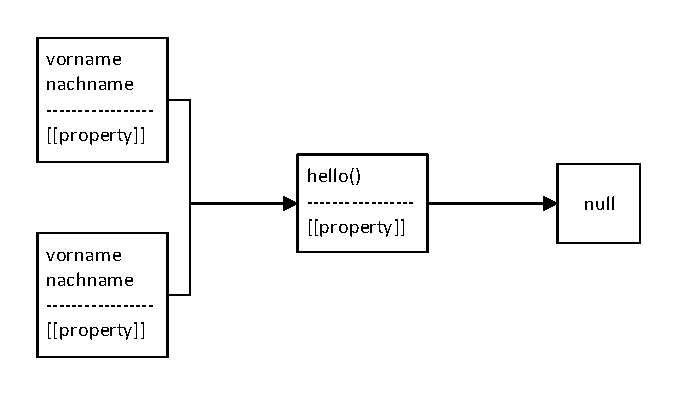
\includegraphics[width=0.7\linewidth]{fig/prototyp}
\caption{Prototyp}
\label{fig:prototyp}
\end{figure}

JavaScript unterstützt JSON von Haus aus. Listing \ref{lst:json} zeigt einige Beispiele zu JSON und Arrays.

\begin{lstlisting}[label=lst:json,caption=JSON]
// JSON.stringify ruft eine Methode toJSON auf (falls diese existiert) und 
// serialisiert das Objekt das zurückgegeben wird
otherModule.toJSON = function(key) {
	var other = {course: this.course, semester: this.semester};
	return other;
}
var otherBachelorModule = JSON.parse(JSON.stringify(otherModule));
console.log(otherBachelorModule);

// Deklaration von Arrays
// Array Literals
var empty = [];
var full = [1,3,8];
var mixed = ["yes", true, 1, 5.0];
var objectArray = [{a:1, b:2}, {a:7,c:15}];

// Array mit new
var another = new Array(); // empty
var oneMore = new Array(5);

// Array Zugriff und Elemente hinzufuegen
var a = ["one"];
console.log(a[0]);
a[1] = "two";
console.log(a.length); // 2

// sparse Array
a[1000] = "thousand"; // Tausendstes Element ist besetzt der Rest ist leer
console.log(a[500]); // undefined

// for loop for sparse arrays
for (var index in a) {
	console.log(a[index]); // one, two, thousand
}

// Weitere Array Methoden -> Buch
// Beispiel reduce (ES5)
var a = [1,2,3,4,5,6];
var sum = a.reduce(function(x,y) {return x+y;}, 0);
console.log(sum); // 21
\end{lstlisting}

In JavaScript sind Funktionen ebenfalls Objekte. Sie erhalten als unsichtbaren Parameter das Keyword \lstinline|this|. Der Wert von \lstinline|this| ist davon abhängig wie die Funktion aufgerufen wird. Listing \ref{lst:methoden-aufruf} zeigt wie Funktionen deklariert und aufgerufen werden. Es gibt vier Möglichkeiten eine Funktion aufzurufen.

\begin{lstlisting}[label=lst:methoden-aufruf,caption=Methoden aufrufen]
// Anonyme Funktion erstellen und an Variable binden
var add = function(a,b) { return a+b; }

// Funktion mit Name an Variable binden (wenn man Funktion rekursiv aufrufen will)
var sub = function sub(a,b) { return a-b; }

// Funktion mit Name ohne an Variable zu binden
function mult(a,b) { return a*b; }

// 1. Funktion mit Name aufrufen
mult(4,5);

// 2. Funktion sofort aufrufen
var fiveToThePowerOfTwo = function(x){return x*x;}(5);
console.log(fiveToThePowerOfTwo);

// 3. Funktion als Literal aufrufen
var aPerson = {
	preName: "Thomas",
	name: "Koller",
	getFullName: function () {
		return this.preName + " " + this.name;
	}
};
console.log(aPerson.getFullName());

// 4. Funktion von anderem Objekt mit apply aufrufen
var dDuck = {
	preName: "Donald",
	name: "Duck"
}

dDuck.getFullName(); // undefined

var donaldsName = aPerson.getFullName.apply(dDuck);
console.log(donaldsName); // Thomas Koller
\end{lstlisting}

In Javascript wird nur pro Funktion ein neuer Scope erstellt. In Listing \ref{lst:scope} werden zwei For-Schlaufen erstellt welche zwei Variablen deklarieren. Eigentlich ist es aber nur eine Variable, weil alle Variablendeklarationen an den Anfang einer Funktion gezogen werden (Hoisting). 

\begin{lstlisting}[label=lst:scope,caption=Scope]
function scopeTest() {
	for(var i = 0; i < 10; i++) {
		console.log(i);
	}
	for(var i = 0; i < 10; i++) {
		console.log(i);
	}
}
// Javascript zieht Variable an den Funktionsanfang (Hoisting)
function scopeTest() {
	var i;
	for(i = 0; i < 10; i++) {
		console.log(i);
	}
	for(i = 0; i < 10; i++) {
		console.log(i);
	}
}
\end{lstlisting}

In JavaScript haben Funktionen Zugriff zum äusseren Scope. Weil auch jede Funktion ein Objekt ist, ist es möglich Closures zu erstellen. Ein Closure kann auch zu einem späteren Zeitpunkt auf seine äusseren Variablen zugreifen, auch wenn dieser Code schon abgearbeitet wurde. Dadurch lassen sich z.B. private Eigenschaften für Objekte erstellen, wie Listing \ref{lst:closure} zeigt.

\begin{lstlisting}[label=lst:scope,caption=Scope]
var myCounter = (function () {
	var value = 0;
	return {
		increment: function (inc) {
			value += inc;
		},
		getValue: function () {
			return value;
		}
	};
}()); // Funktion wird sofort aufgerufen

myCounter.increment(10);
console.log(myCounter.getValue()); // 10
console.log(myCounter.value); // undefined
\end{lstlisting}

Ein Vorteil von Java ist die Objektorientierung und auch die literale Syntax um Objekte zu erstellen. Auch Closures kann man ohne Probleme verwenden. Man sollte darauf achten dass man immer mit \lstinline|===| und nicht mit \lstinline|==|, sonst werden die Werte komisch umgewandelt. Auch die Verwendung von Prototypen und \lstinline|with| sollte man vermeiden. Besondere Vorsicht ist bei globalen Variablen, dem Scope und den Einfügeregeln von Semikolons geboten. Auch das Schlüsselwort \lstinline|typeof| und \lstinline|eval| sind nicht zuverlässig.